\documentclass[conference]{IEEEtran}
\IEEEoverridecommandlockouts
% The preceding line is only needed to identify funding in the first footnote. If that is unneeded, please comment it out.
\usepackage{cite}

\usepackage{amsmath,amssymb,amsfonts}
\usepackage{algorithmic}
\usepackage{graphicx}
\usepackage{textcomp}
\usepackage{xcolor}
\usepackage{pifont}
\usepackage{float}

\newcommand{\xmark}{\ding{55}}%
\newcommand{\cmark}{\ding{51}}%

\def\BibTeX{{\rm B\kern-.05em{\sc i\kern-.025em b}\kern-.08em
    T\kern-.1667em\lower.7ex\hbox{E}\kern-.125emX}}
\begin{document}

\title{A Simulation Study of Hardware Parameters for GPU-based HPC Platforms
%{\footnotesize \textsuperscript{*}Note: Sub-titles are not captured in Xplore and
%should not be used}
%\thanks{Identify applicable funding agency here. If none, delete this.}
}

\author{\IEEEauthorblockN{Saptarshi Bhowmik}
\IEEEauthorblockA{
\textit{Florida State University}\\
bhowmik@cs.fsu.edu}
\and
\IEEEauthorblockN{Nikhil Jain}
\IEEEauthorblockA{
\textit{NVIDIA Inc.}\\
nikhijain@nvidia.com}
\and
\IEEEauthorblockN{Abhinav Bhatele}
\IEEEauthorblockA{
\textit{University of Maryland}\\
bhatele@cs.umd.edu}
\and
\IEEEauthorblockN{Xin Yuan}
\IEEEauthorblockA{
\textit{Florida State University}\\
xyuan@cs.fsu.edu}
}

\maketitle

\begin{abstract}
  High Performance Computing (HPC) platforms are switching to GPU-based compute nodes;
  the resulting trend is the increase in per node computational capacity
  and the reduction of the number of endpoints in the system. This trend changes the
  computation and communication balance in comparison to the pre-GPU era HPC platforms,
  which warrants a re-study of the hardware architectural parameters. In this research,
  we perform a simulation study of the impact of crucial hardware  parameters
  in GPU-based systems using HPC workloads that consist of representative
  HPC applications. The hardware parameters studied include (1) link bandwidth, (2) number
  of GPUs per node, and (3) interconnection network topology.
%  
%  in an interconnect network, more number of
%  HPC Platforms are switching to GPU based compute nodes. However, the actual performance
%  of HPC system all together, is affected by various other environment and hardware
%  parameters. Here, in this poster we are studying the effect of one crucial hardware
%  parameter 1) Link Bandwidth and one simulation environment of 2)GPUs per node,
%  on the performance of few common HPC applications, in the context of two
%  popular topology - Fat Tree and Dragonfly.  
\end{abstract}

\begin{IEEEkeywords}
  GPU clusters, computation and communication balance, hardware parameters, performance. 
\end{IEEEkeywords}

\section{Introduction}

GPUs are increasely used in High Performance Computing (HPC) platforms. A compute node
in high-end HPC systems often has multiple GPUs. The resulting trend
is the increase in per node computational capacity and the decrease in the number
of endpoints in the system -- the computation and communication ratio in such systems
is different from that in pre-GPU era platforms. For a GPU-based platform to achieve
high performance, it is imperative that computation and communication in the system
to remain balanced. Important hardware architectural parameters such as the
link bandwidth and the number of GPUs per node are crucial design parameters that will
determine the balance and thus, the overall performance of the system. In this research,
we leverage the whole system simulation capability of TraceR-CODES \cite{b4} and use it
to study the impact of hardware parameters using HPC workloads that consist of
representative HPC applications. The parameters studied include
(1) interconnect link bandwidth, (2) number of GPUs per node, and (3) interconnect topology.
The study gives insight of the hardware parameters and the results can be used to guide
the design of GPU-based HPC platforms. 

%Currently deployed networks are trying to reduce the number of
%endpoints by leveraging the GPU based compute nodes. These new GPU
%based compute nodes have larger computational prowess compared to a traditional
%CPU based compute nodes. However, there has been a continual discrepancy of
%computation and communication performance, with later, growing at a much slower rate.
%Along with that, increasing number of modern accelerations further dwindles this ratio.
%As such, there is a need to identify the environment and hardware specifications to make
%best possible use of the available system, and have a ideal communication/computation
%balance.  

\section{Methods}

We use the discrete event driven simulator, TraceR-CODES\cite{b4} for the study.
TraceR-CODES is capable of simulating the whole system with different hardware parameters.
Moreover, it can simulate a workload in the system that consists one
or multiple applications by replying the traces of the applications. 

\subsection{Applications and Workloads}

We select 6 representative applications for our experiments that include two computation
intensive kernels Kripke and Laghos, two communication kernels Stencil4d and Subcomm, and
two applications Sw4lite and Amg  that have a mixed of communication and computations. 
We profile and collect the traces for these applications of different ranks
using Score-P\cite{b3}. The applications are summarized in Table~\ref{tab1}.

We are running 20 Workloads of randomly selected jobs from the six applications listed
in Table~\ref{tab1}, from ranks 32, 64, 128, 256 and 512, to fill up the whole system.
We make sure that each rank of an application appears at least 4 times throughout all
the 20 workloads.

\begin{table}[htbp]
\caption{Application Traces}
%\begin{adjustbox}{width=\columnwidth,left}
\begin{center}
  \begin{tabular}{|c|c|c|} \hline
\hline
\textbf{Traces} & \textbf{Computation} & \textbf{Communication} \\ \hline
Stencil4d & \xmark & \cmark  \\    \hline
Kripke & \cmark & \xmark  \\    \hline
Laghos & \cmark & \xmark  \\    \hline
Subcomm-a2a & \xmark & \cmark  \\    \hline
Sw4lite & \cmark  & \cmark  \\    \hline
Amg & \cmark  & \cmark  \\    \hline
\end{tabular}
\label{tab1}
\end{center}
\end{table}
  
\subsection{Network Topologies}

We use two popular interconnect topology 1D-Dragonfly and Fat-Tree for all our
simulation\cite{b5}. For 1D-Dragonfly, we start our simulation with 16 groups and
1 GPU per compute node. We then reduce the size of the network to 8 group for
2 GPUs per compute node, 4 group for 4 GPUs per compute node and 1 group for
8 GPUs per compute node. For Fat-Tree, we start with 8 pods for 1 GPU per compute
node  and keep on reducing the number of pods as we increase the number of GPUs
per compute node. Ultimately have four configurations for Fat-Tree 8 pods for 1
GPU per compute node, 4 pods for 2 GPU per compute node, 2 pods for 4 GPU per
compute node and 1 pods for 8 GPU per compute node. ****** how many total nodes, and nodes
per group or pod ******

\subsection{Bandwidth}

We set the base bandwidth(x) for the Links as 11.9 Gb/s, which is the link
bandwidths used in Quartz machines, and keep the internal bandwidth as 23.8 GB/sec.
We use 8 more bandwidth, x/16, x/8, x/4, x/2, 2x, 4x, 8x, 16x,  which are a proportion
of the base bandwidths, for our simulations.

\subsection{GPUs per node}
 
We are using 1 GPU per node for a maximum sized network and then we are subsequently
increasing it to 2 GPUs per node, 4 GPUs per node and 8 GPUs per node, with
reducing the network size simultaneously. 

\section{Results and conclusions}

\subsection{Impact of GPUs per Node}\label{AA}

Figure~\ref{gpu1} shows the application speedup with respect to the default setting of
1 GPU per Node with the default link bandwidth (1x) on 1D-Dragonfly. As the total number of
GPUs condense to a smaller number of compute nodes, the performance of communication kernels
(stencil4d and subcomm)
drops significantly while the performance of computational intensive kernels
(Kripke and Laghos) remains the similar. The performance of applications (Amg and Sw4lite)
is also affected as shown in the figure. The results on fat-tree have a similar trend
and are omitted. 

\begin{figure}[H]
\centering
\centering
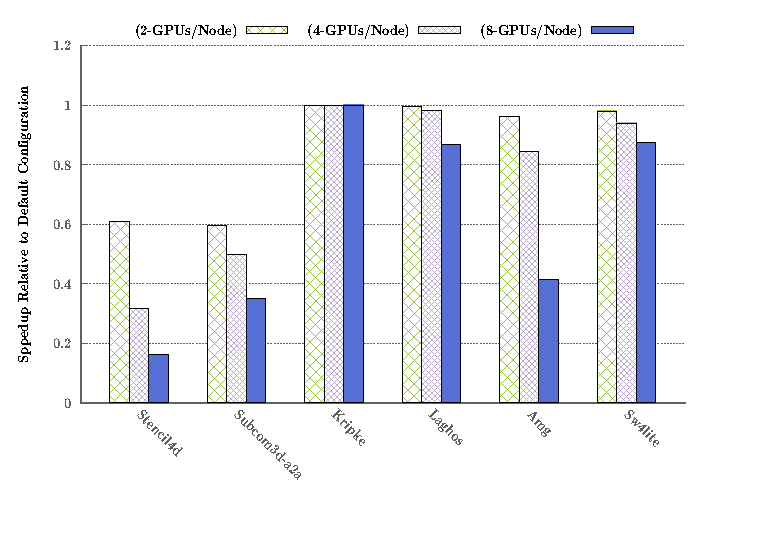
\includegraphics[width=1\linewidth, height=5cm]{figs/dfly-x-mapping-all.eps}
%\captionsetup{labelformat=empty}
\vspace{-0.15in}
\caption{Different GPUs per node mapping for all Applications of 128 ranks in 1D-Dragonfly}
\label{gpu1}
\end{figure}

%\begin{figure}[H]
%\centering
%\centering
%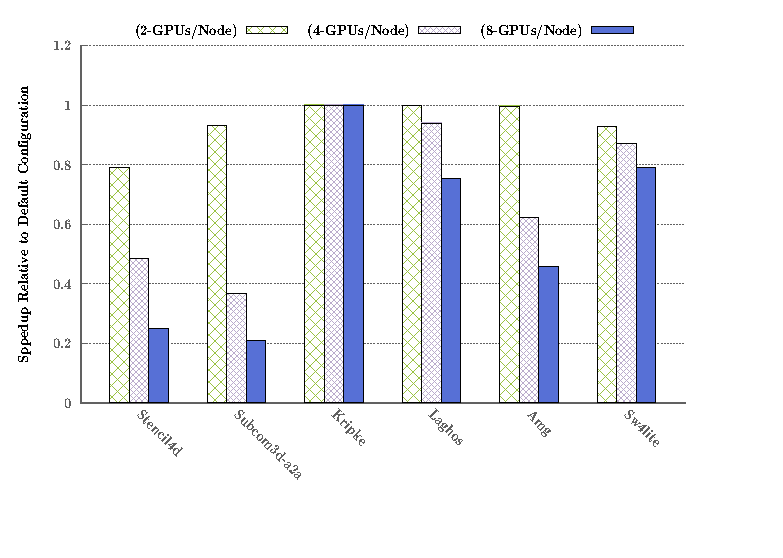
\includegraphics[width=1\linewidth, height=5cm]{figs/ftree-x-mapping-all.eps}
%%\captionsetup{labelformat=empty}
%\caption{Different GPUs per node mapping for all Applications of 128 ranks in Fat-Tree}
%\end{figure}
%
%Communication intensive applications experience more slowdown than applications with computation.

\subsection{Impact of Bandwidth}

Figure~\ref{bw1} shows application speedup with respect to the default setting is 1 GPU
per Node and Link Bandwidth 1x (11.9 Gb/s) on 1D-Dragonfly.  
There are two key observations. First, for applications that are sensitive to communication
performance (Stencil4D, subcomm, Amg, and Sw4lite), as the number of GPU per node
increases, more link bandwidth is needed to sustain the performance -- insufficient bandwidth
will significantly slow down the applications. This is even observed in the computation
intensive Laghos. Second, every application has a sweet spot where it is performing the
best. This indicates that substantial benchmarking study will be needed to determine the
best system configurations for the GPU-based systems. Figure~\ref{bw2} shows the results with
the fat-tree topology, the trend is the same. Thus, these conclusions apply across
topologies. 

\begin{figure}[H]
\centering
\centering
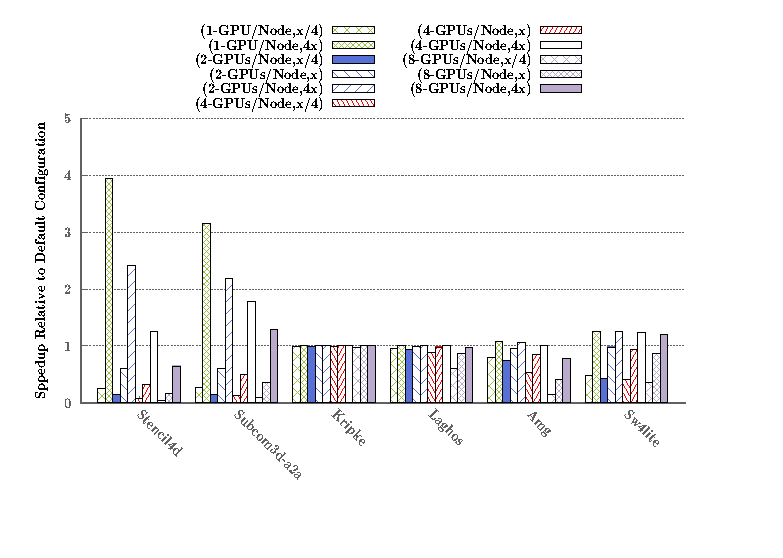
\includegraphics[width=1\linewidth, height=5cm]{figs/dfly-bw-mapping-all.eps}
%\captionsetup{labelformat=empty}
\vspace{-0.15in}
\caption{Different Bandwidth and GPUs per node mapping for all Applications of 128 ranks in 1D-Dragonfly}
\label{bw1}
\end{figure}

\begin{figure}[H]
\centering
\centering
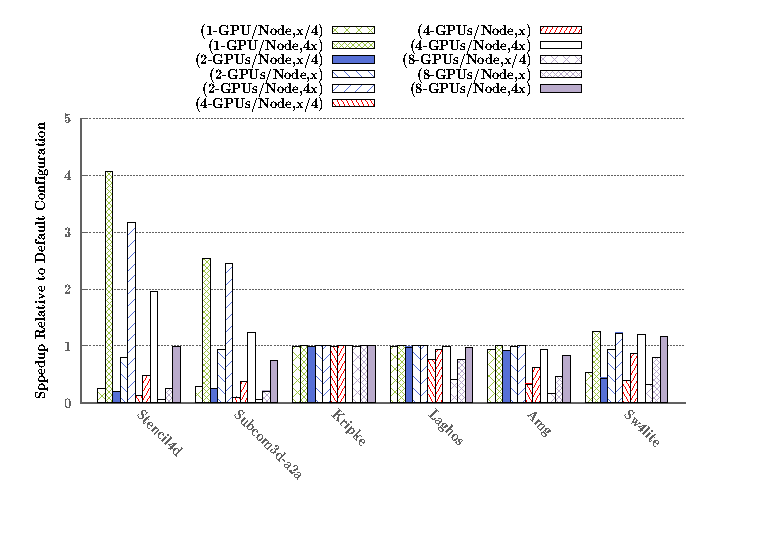
\includegraphics[width=1\linewidth, height=5cm]{figs/ftree-bw-mapping-all.eps}
%\captionsetup{labelformat=empty}
\vspace{-0.15in}
\caption{Different  Bandwidth and GPUs per node mapping for all Applications of 128 ranks in Fat-Tree}
\label{bw2}
\end{figure}

\section{Conclusions and Future Works}

We perform a simulation study of hardware Parameters for GPU-based HPC Platforms. What
differentiates our study from others is that we use workloads consist of representative
applications. Our results shed lights into the impact of hardware parameters on real
applications. In the future, we plan to extend the study by (1) considering other
interconnect choices, (2) using more applications, and (3) study other system parameters.

%\begin{itemize}
%    \item Study how other simulation environment and hardware design, such as NIC scheduling %policies effect the performance of applications
%
%    \item Profile more HPC applications and find the performance of those applications across% the currently deployed GPU based interconnect topology,
%\end{itemize}


\begin{thebibliography}{00}

\bibitem{b1} Jain, N., Bhatele, A., Howell, L. H., Böhme, D., Karlin, I., León, E. A., et al. (2017, November). Predicting the performance impact of different fat-tree configurations. In Proceedings of the International Conference for High Performance Computing, Networking, Storage and Analysis (pp. 1-13).
\bibitem{b2} Kim, J., Dally, W. J., Scott, S., and Abts, D. (2008, June). Technology-driven, highly-scalable dragonfly topology. In 2008 International Symposium on Computer Architecture (pp. 77-88). IEEE.
\bibitem{b3} Knüpfer, A., Rössel, C., an Mey, D., Biersdorff, S., Diethelm, K., Eschweiler, D., et al. (2012). Score-p: A joint performance measurement run-time infrastructure for periscope, scalasca, tau, and vampir. In Tools for High Performance Computing 2011 (pp. 79-91). Springer, Berlin, Heidelberg.
\bibitem{b4} Acun, B., Jain, N., Bhatele, A., Mubarak, M., Carothers, C. D., and Kale, L. V. (2015, August). Preliminary evaluation of a parallel trace replay tool for hpc network simulations. In European Conference on Parallel Processing (pp. 417-429). Springer, Cham.
\bibitem{b5} Alzaid, Z. S. A., Bhowmik, S., Yuan, X., and Lang, M. (2020, June). Global link arrangement for practical Dragonfly. In Proceedings of the 34th ACM International Conference on Supercomputing (pp. 1-11). Magnetics Japan, p. 301, 1982].

\end{thebibliography}
\vspace{12pt}
\end{document}
